\documentclass[12pt]{article}
\usepackage{titling}
\newcommand{\subtitle}[1]{%
  \posttitle{%
    \par\end{center}
    \begin{center}\large#1\end{center}
    \vskip0.5em}%
}
\usepackage{array}
\setlength\extrarowheight{2pt}
\usepackage{CJKutf8}
\usepackage{apacite}
\usepackage{bigints}
\usepackage{amsmath}
\usepackage{amssymb,enumerate}
\usepackage{bibentry}
\usepackage{caption}
\usepackage[authoryear,round,longnamesfirst]{natbib}
\usepackage{setspace}
\linespread{1.5}
\usepackage{enumitem}
\usepackage{graphicx}
\usepackage{epstopdf}
\usepackage{etoolbox}
\AtBeginEnvironment{quote}{\singlespacing\small}
\usepackage{float}
\usepackage{framed}
\usepackage{geometry}
\usepackage{graphicx}
 \geometry{
 a4paper,
 total={210mm,297mm},
 left=25mm,
 right=25mm,
 top=25mm,
 bottom=25mm,
 }
\usepackage{pdflscape}
\usepackage{array}% http://ctan.org/pkg/array
\usepackage{color, colortbl}
\definecolor{Gray}{gray}{0.95}
\definecolor{LightGray}{gray}{0.85}
\definecolor{VLightGray}{gray}{0.75}
\definecolor{darkblue}{rgb}{0.0,0.0,.7}
\definecolor{shadecolor}{gray}{0.85}
\usepackage{color}
\DeclareUnicodeCharacter{00A0}{ }
\usepackage{hyperref}
\hypersetup{colorlinks,breaklinks,linkcolor=darkblue,urlcolor=darkblue,anchorcolor=darkblue,citecolor=darkblue}
\usepackage{wrapfig}
\newcommand{\zh}[1]{\begin{CJK}{UTF8}{gbsn}#1\end{CJK}}

\usepackage{setspace}
\usepackage{epigraph}
\usepackage{titling}

\usepackage{etoolbox}
\AtBeginEnvironment{quote}{\singlespacing\small}

\setlength{\droptitle}{-4em}
\setlength\epigraphwidth{16cm}
\setlength\epigraphrule{0pt}

\interfootnotelinepenalty=10000

\title{Who Not What: \\ \large The Logic of China's Information Control Strategy\thanks{We are very grateful to Martin Dimitrov, Iza Ding, Jennifer Earl, Dimitar Gueorguiev, Jeffrey Javed, Kevin O'Brien, and Rachel Stern for comments on earlier drafts of this paper and to the participants of workshops at the Hertie School of Governance, the Fairbank Center for Chinese Studies, and at Hamilton College for feedback. This work was funded by doctoral student grants from the Lieberthal-Rogel Center for Chinese Studies and the Department of Political Science at the University of Michigan.}}

\author{Mary\ Gallagher\thanks{\normalsize Professor, Department of Political Science, University of Michigan, Haven Hall, Ann Arbor, MI 48109-1045 (E-mail: \mbox{metg@umich.edu}).} \and Blake\ Miller\thanks{\normalsize Corresponding author,
    Department of Methodology, London School of Economics and Political Science, Columbia House, Aldwych, London WC2A 2AE (E-mail: \mbox{b.a.miller@lse.ac.uk}).}}

\date{\today\vspace{1em}\\}

\begin{document}

\begin{CJK*}{UTF8}{gbsn}
\maketitle\vspace{-2em}
{\setstretch{1}
\begin{abstract}
In this paper, we examine how the Chinese state controls social media. While social media companies are responsible for censoring their platforms, they also selectively report certain users to the government. Our focus in this article is to understand the logic behind media platforms' decisions to report users or content to the government. We find that content is less relevant than commonly thought. Information control efforts often focus on {\it who} is posting, rather than {\it what} they are posting. The state permits open discussion and debate on social media while controlling and managing influential social forces that may challenge the Party-State's hegemonic position. We build on ``ideology and organization'' by \cite{schurmann1968ideology}, emphasizing the Party's goals of embedding itself in all social structures and limiting the ability of non-Party individuals, networks, or groups to carve out separate space for leadership and social status. In the virtual public sphere, the Chinese Communist Party (CCP) continues to apply these principles to co-opt, repress, and limit the reach of influential non-Party ``thought leaders.'' We find evidence to support this logic through qualitative and quantitative analysis of leaked censorship documents from a social media company and government documents on information control.\\

\begin{center}
    {\bf 摘要:}
\end{center}

此论文探讨中国政府如何控制社交媒体。社交媒体公司不仅负责审查自身平台,也会有选择性地向政府部门上报一些用户。此论文重点研究媒体平台上报用户或内容背后的选择逻辑。我们发现媒体对内容的审查并非如过往研究发现的那么重要。信息审查通常更着眼于发布者是谁,而不是发布者说了什么。中国政府允许社交媒体上的公开讨论和辩论,而同时控制和管理可能挑战党国领导权的意见领袖和有影响力的社会势力。我们的研究基于舒尔曼的《共产主义中国的意识形态和组织》。舒尔曼强调党的目标是将自身融入所有社会结构,并限制其他个人或团体能占领的公共空间。中国共产党根据这些原则来吸纳,压制和限制体制外“意见领袖”在网络公共空间里的影响力。我们使用定性与定量分析研究一整套被泄露的新浪微博审查文件和一整套思想工作干部指南,分析结果证实了我们的理论。\\

\noindent{\bf 关键词:} 社交媒体; 意见领袖; 压制; 审查
\end{abstract}
}
\newpage

\section*{Introduction}

\paragraph{} Neihan Duanzi (neihan duanzi, 内涵段子) was a seemingly harmless social media portal for videos, memes, and jokes in China, similar to Reddit or 4chan. It rarely hosted criticisms of the government or calls for collective action. However, as the site gained popularity, users began to form offline communities, meeting up and identifying each other in public, sometimes communicating in secret codes of car honks at intersections. In April of 2018, the government surprised many by shutting the site down. We argue that this decision reflects the regime's strategy of maximally shrinking non-official public spaces that could threaten the CCP's authority or compete with it ideologically in the future. Neihan Duanzi's large and growing community was not a clear threat to the CCP at the time of its ban, but it had the potential to transform into one. Using the example of another platform, Sina Weibo (xinlang weibo, 新浪微博), we argue that the key to shrinking this space is the careful targeting of individuals who are influential within counter-hegemonic spaces such as Neihan Duanzi.

\paragraph{} While the state could reassert control over these spaces by shuttering all private social media platforms, it benefits from a well-maintained and constrained private media ecosystem. The Chinese state, once at odds with capitalism, is now using it as a source of stability. Drawing on the expertise of tech firms who continue to innovate in social networks, digital payments, and targeted advertising analytics, the government can reserve real-world and violent repression for those who are flagged by algorithms predicting future acts of state subversion. These systems are already in development \citep{merics2017social,yang2017social}. Through co-optation of technology companies, the state enforces information control and repression with a scalpel rather than a hammer. 

\paragraph{} The Chinese state has carefully constructed its repression regime to tame citizens via impersonal censorship algorithms, calibrating, and customizing its tactics for different individuals and contexts. For many, the intrusion of state security into their lives is merely virtual and often covert and unobserved. For a select few who dare to push the boundaries, online censorship may be more explicit and threatening. It may also move from the virtual realm to real-world interaction---home visits, invitations to ``drink tea,'' interrogations, detentions in a black jail, or worse.

\paragraph{} We analyze when delegated, sometimes automated, censorship of online content shifts back to the state's repressive apparatus. The Chinese government delegates online censorship to private internet content producers (ICPs) like Sina and Tencent, and compels them to satisfy the government's demand for information control. While much of the work of delegated censorship is the deletion or hiding of sensitive content, ICPs also selectively report certain content and users back to the government. We seek to understand the logic of this reporting system: who and what are targeted for handling by the state itself?
 
\paragraph{} We find that ``reporting up''---which likely results in direct state repression or co-optation---is targeted toward influential public opinion leaders whose standing and influence may threaten the Party's hegemonic presence in China's online public sphere. Substantive topics, though relevant, matter less than user influence and virality in state efforts to ``guide opinion'' through direct repressive interventions. Many topics---including topics that have an apparent collective action threat (a political dissident, a workers' strike)---are not reported up unless they achieve a certain degree of virality or influence. By contrast, many viral discussions that challenge the legitimacy of the regime in more indirect and oblique ways (elite defection, ridicule of top leaders) are reported up.
 
\paragraph{} Work by \cite{schurmann1968ideology} speaks to the state logic of ``who not what.'' In his work on the early years of CCP rule, he emphasizes the importance that the CCP placed on ideology and organization in its social revolution, which he conceptualized as a process of destruction and replacement of former elites. Communist control had both ideational and spatial dimensions. Ideology replaced other values and norms of China's old society. Communist organization embedded the party in all social, economic, and political structures and eliminated the old elite, from landlords to factory owners. However, in the second edition of Ideology and Organization, Schurmann's analysis of the Maoist state during the Cultural Revolution is instructive for understanding how Maoism approaches challenges of a new, emerging elite. In Schurmann's analysis, social mobilization, especially of students in the Cultural Revolution, challenged the CCP's organizational dominance. ``If power is the key element in organization, authority is the key element in a social system'' \citep[521]{schurmann1968ideology}.  

\paragraph{} The contemporary context is quite different from that of the late 1960s. However, the emergence of a dynamic private sector, new social classes, and independent sources of wealth and social status poses similar challenges to the CCP's organizational dominance. In private firms, especially recently, the CCP has attempted to establish and strengthen the role of Party cells. In social media, however, organizational dominance is not possible. Instead, the CCP has developed tactics to reduce the authority of new voices, to limit their virality, and to eliminate or co-opt alternate sources of leadership and influence. The battle for online public opinion dictates an ambitious approach that seeks to allow for online expression while also suppressing the rise of influential voices and viral discussions. Although the government is worried about the Internet as a device to facilitate social movements and protests, it also worries simply when a large number of people online are talking about the same thing, what it calls ``a public opinion emergency'' (gonggong yulun weiji, 公共舆论危机) or an ``internet opinion emergency'' (wangluo yulun weiji, 网络舆论危机). Schurmann notes that in the context of an evolving social system, in which Communist organization is either not complete or weakened, authority is crucial. Controlling, managing, co-opting authoritative voices online is critical. 

In social movement theory, authoritative actors can play the role of brokers in the diffusion of social mobilization, protest, and other forms of collective action. These influential actors serve as nodes in networks that may then connect up. In his  study of  transnational activism, Tarrow defines brokerage as ``linking of two or more previously unconnected social actors by a unit that mediates their relations with one another and/or with yet other sites'' \citep[190]{tarrow2005new}. In social media interaction, Big V-users can easily link up users who previously had no connection to each other, spawning information cascades and viral discussions of hot topics. As we show below, the government is especially worried about viral discussions sparked by influential thought leaders.

\paragraph{} The state's evolving response to social grievances since the violent suppression of the student movement in 1989 can help us understand the tension between increased openness of communication and the state's goal of maintaining hegemony over discourse. Responding to the mistakes of 1989, the Chinese state developed a new toolkit---often called ``responsive authoritarianism''---that combines targeted repression and broad responsiveness. It has become more tolerant of narrowly-expressed, localized, and economistic protests and grievances. At the same time, its ability to target and isolate political dissidents and to use repression to silence the regime's most vociferous opponents has improved. With the explosion of social media since 2009, however, it has become more challenging for the state to prevent online publics from broadening beyond initially narrow grievance articulation. The networked and rapid nature of discussion online can unite similarly-aggrieved individuals across time, space, and barriers of region, class, and even language. For example, local scandals in food safety, wage arrears, or corruption can be more easily linked to systemic problems in the authoritarian political system, such as the lack of a free press, independent trade unions, or close relations between political and business elites. Social media has the potential to transform narrow, local problems to broad, system-challenging threats.
 
\paragraph{} Maintaining responsiveness while containing the threat of the online public sphere is a delicate balancing act. To maintain its responsiveness, which seems to have vastly improved the government's legitimacy \citep{nathan2003authoritarian,dickson2016dictator,tang2016populist,zhang2017reza}, the central government uses social media discussion to monitor its local agents and mitigate the severe principal-agent problems inherent in China's top-down system. Ever concerned with information cascades that may lead to collective action \citep{kuran1991now, lohmann1994dynamics, denardo2014power}, the government seeks to prevent social media from acting as the ``single spark that ignites a prairie fire'' by controlling the virality influence of public opinion leaders online. CCP manuals to train Internet censors specifically reference this problem as the ``butterfly effect'' (hudie xiaoying, 蝴蝶效应), the need to control information before it gets out of (their) control \citep{wei2015gongan,gao2011wangluo,zou2015wangluo,guowuyuan2016guowuyuan}.
 
\paragraph{} This article has four parts. In the first section, we examine control dynamics over time, arguing that the regime has moved from broad-based repression to targeted repression coupled with responsiveness to a broader swathe of the population.  The second section uses government manuals and documents on opinion guidance and internal censorship logs from a social media company to analyze when commercial censors report users and information back up to the government. These sources allow us to both quantitatively test our model and supplement our results with additional transcript evidence from government sources \citep{doi:10.1177/0951629816664420}. The third and final section discusses the findings.

\section{The Rise of Responsive Authoritarianism and the Challenge of Virality}

\paragraph{} The Chinese Communist Party's approach to socio-political control has shifted over time. As economic reforms sped up in the 1990s, the government became far more tolerant toward protests that it saw as rooted in socio-economic grievances brought on by market reform. Small and narrow protests multiplied during this time, with protestors limiting their claims and often hiding organizations and leaders. These protests were different not only in who participated, but also in their claims, their targets, and their tactics. On the other side, the government began to overhaul the repressive apparatus of the state to improve its ability to preempt significant challenges while placating reasonable grievances \citep{tanner2004china}.

\paragraph{} Protesters often framed their grievances as narrow and economistic. They focused on economic deprivation and loss precipitated by the disruptive and destabilizing economic restructuring and often unregulated growth. These protests overwhelmingly, and perhaps even intentionally, articulated their targets as bad local actors, such as corrupt local officials, greedy enterprise bosses, or compromised local bureaucrats who failed to enforce central laws strictly when such laws interfered with growth. These lower-level targets were best attacked using tactics that were wholeheartedly moralistic and normative, but also, at times, legalistic. As \cite{obrien2006rightful} have described, their invocation of resistance was rooted in support for the legitimate policies and laws of the central government and their anger that local governments did not enforce them. Demands were for better rule, not for a new set of rulers.

\paragraph{} The turn toward increased state-society dialogue has been labeled bargained authoritarianism \citep{lee2013power}, responsive authoritarianism \citep{heurlin2017responsive}, and contentious authoritarianism \citep{chen2012social}. These terms---though they emphasize different aspects of the phenomenon---hone in on the notion of protest as an accepted mode of political participation in contemporary China \citep{tang2016populist}. State and society have both learned new tactics to make high levels of protest in an authoritarian regime sustainable, yielding neither to mass repression or a tipping point toward revolution \citep{heurlin2017responsive,lee2013power,su2010street,cai2008local}. In this game of cat and mouse between state and society, citizens became adept at constrained escalation, normative morality plays, and hiding the degree to which protests had leaders or organizational capacity to avoid the most severe repression \citep{o2015repression,fu2017disguised}.

\paragraph{} The Chinese state has not eliminated repression from its tool kit during this period of responsive authoritarianism. Instead, repressive tactics have become more targeted, hidden, pre-emptive, and psychologically sophisticated \citep{ong2015thugs,chen2017origins,cai2008local}. Deng and O'Brien examine the practices of ``psychological coercion'' and ``relational repression'' as strategies deployed by state agents who find it harder to dominate through sheer physical coercion or have lost the ability to withhold resources, especially to citizens with their market power. An aggrieved citizen might discontinue resistance at the insistence of colleagues or relatives \citep{o2015repression, deng2013relational}. \cite{o2017preventing} note that ``protest control is taking on a person-by-person quality'' made possible by the vast increase in state resources dedicated to internal security and stability \citep[see also][]{wang2015rise,ong2015thugs}.

\paragraph{} China's progression toward more sophisticated repressive strategies is not unique. In many parts of the world, the use of non-physical, hidden, or delegated repression is widespread \citep{earl2003tanks}. \cite{davenport2007state} shows how high capacity states can disable social movements without overt violence. \cite{frantz2014dictator} find that the ability to co-opt potential opposition leaders can alter an authoritarian government's need for widespread repression while enhancing their ability to target opponents of the regime. Sophistication and ``person-to-person'' contact are not cheap. Observers noted in 2011 that China's internal security budget exceeded its spending on the military. \cite{wang2015rise} detail the ``rise of the security state'' and its multiple tasks of bargaining, compensation, surveillance, and repression.

\paragraph{} Escalation incentives are baked into the model of responsive authoritarianism \citep{tanner2004china,chen2012social,cai2010collect,o2015repression}. This is evident from a pithy saying used by protesters: ``Do nothing and get no results, do something small and get small results; do something big, and get a big result'' \citep{tanner2004china}. With the rise of social media, escalation has become far easier with lower costs and more immediate impact. Online discussions can aggregate narrow and limited grievances (e.g., environmental degradation, food safety, or lapses in public safety) into encompassing demands for greater transparency, a freer media, or bottom-up accountability for political elites. Netizens with large followings and influence on social media can rapidly bring these encompassing demands into the public discourse.

\paragraph{} Responsive authoritarianism has also clearly benefited the government. Since 1989, it has gained legitimacy from its more accommodating stance toward protest and grievances \citep{dickson2016dictator,tang2016populist}. Social media also provides the central government easier access to ``real'' public opinion, solving the ``dictator's dilemma'' of not having a true sense of how people feel about a repressive regime \citep{wintrobe2000political}. If people feel like they can be more honest in social media, the regime also benefits informationally. How can the government have its cake and eat it too? How can it sustain high levels of protest and response/bargaining within the context of extensive social media use? Can responsive authoritarianism survive the onslaught of virality?

\section{Empirical Analysis}

\paragraph{} We draw upon two sources of data: 1) government documents and manuals about ``opinion guidance,'' and 2) leaked internal documents from a social media company, Sina Weibo. The former serves as transcript evidence: a record from the government of its logic of control. The latter empirically tests our theory of information control using a model of the decisions of a popular Twitter-like social networking site, Sina Weibo, to escalate users and content on their platform to relevant authorities.
\paragraph{} These leaked internal censorship documents help us test our theory of what kind of online content and users are relayed back to the government by media companies. It is evident from government documents and manuals analyzed in this paper that government outreach to social media ``thought leaders'' involves a combination of carrots and sticks.
\paragraph{} Evidence from our analysis suggests that the state is most worried about controlling the virality of content, the influence of individuals, and the ability of social media discussion to mobilize and incite. In order to reduce the virality of a discussion or shape the course of a discussion, the state eliminates certain types of posts, reduces the influence of opinion leaders, and gives a freer rein to the ``nobodies'' (for example, by allowing small users more leeway than big users).

\subsection{Evidence from Government Documents}

\paragraph{} In this section, we present transcript evidence of the state's logic of information control: to focus repressive activities on influential users rather than categories of content. This section draws on data from dozens of Party- and government-produced books, documents, or manuals about ``opinion guidance,'' ``thought work,'' and information control, whose intended audience is government leadership cadres. The authors of these sources are high-level propaganda and public security officials, as well as government-affiliated academics.
\paragraph{} Government logic of opinion guidance described in these manuals is consistent with our theory of ``who not what.'' These documents show that the state focuses its opinion guidance efforts on users with large followings or viral posts: ``opinion leaders'' (yijian lingxiu, 意见领袖). Most opinion guidance manuals included at least a small section devoted to managing these ``opinion leaders.'' Below, we will present this logic using excerpts from government manuals and documents.
\paragraph{} Manuals suggest that the Party is concerned that it has ceded too much discourse power to voices outside the system. One manual suggests, ``the mechanism for public opinion formation online has changed... [as the] means of digital dissemination has broken the [state's] traditional monopoly of discourse.'' This manual laments that social media has ``brought about a change of position from strong to weak among elites, and from weak to strong among the grassroots.'' It suggests,  ``because cyberspace has no systemic barriers or binding ideological constraints, all kinds of thoughts, ideas, and values have a platform. Different classes, areas, and types of media can exchange, integrate, or confront these ideas, making the public opinion environment increasingly complex'' \citep[118-122]{zhou2011weibo}. In excerpts presented later in this section, the state appears fearful of opinion leaders' ability to organize individuals around counter-hegemonic ideas. They suggest that in order to confront the expanded space for counter-hegemonic discourse brought by the internet, cadres must engage with opinion leaders who occupy the most social real-estate in the online opinion field. Manuals direct cadres to pay particular attention to ```Big V' users who have many fans and followers... [because they] decide the development of online opinion events or the formation of topics of discussion'' \cite[180-194]{zeng2015wangluo}.
\paragraph{} Manuals not only consistently stress the importance of opinion leaders in the state's opinion guidance efforts, but they also agree about the metrics cadres should use to track and identify them. One manual suggests the importance of two key metrics: repost counts and fan/friend counts. This manual suggests, ``Weibo's special model for information dissemination makes it much easier for social media surveillance workers to identify opinion leaders and the original source of opinions'' \citep[201-228]{zhou2011weibo}. Another manual elaborates on the logic behind targeting users based on these variables, citing internal government research on Weibo:

\begin{quote}
``[In] over 30 viral opinion incidents on Weibo between 2011 and 2012, there were only 7584 viral posts where the number of retweets surpassed 500; a mere 305 Weibo users authored 5047 of these posts. Moreover, these 5047 posts [were the root source of] 66.5\% of all total posts and 80\% of all retweets and comments. Though the public opinion space seems complex and untenable, in reality, it is largely controlled and led by a small number of big V users...'' \citep[180-194]{zeng2015wangluo}.
\end{quote}

\paragraph{} In this same manual, the authors suggest that the state should balance their dual goals of responsiveness and control by regularly approaching opinion leaders, guiding them toward consensus and learning from their perspectives:

\begin{quote}
``We must communicate with them, seek consensus, and let them make suggestions from a rational and constructive perspective, instead of publishing aggressive and inflammatory extreme speech as they please [...] it is necessary to maintain close contact with them, through regular or irregular meetings or online exchanges, to take the initiative to invite them to visit major public projects...'' \citep[180-194]{zeng2015wangluo}. 
\end{quote}

\paragraph{} The manuals suggest that the state is keenly aware of the agenda-setting power and social import of celebrities, intellectuals, and artists online \citep[115-123]{dang2013wangluo}. These individuals can ``set a new agenda to lead the public to focus their attention elsewhere, resulting in a change in the overall direction of public opinion'' \citep[201-228]{zhou2011weibo}. One manual discusses the case of a 2010 Shanghai high-rise fire that killed 58 people. It suggests, ``changes in the agenda of discussion of this event were closely related to the actions of opinion leaders.'' In the aftermath of the disaster, celebrity blogger Han Han (韩寒) and other famous journalists brought to light systemic issues behind the high-rise fire on social media platforms. Public outcry reached a fever pitch after a popular blogger organized a ``public mourning event that attracted 100,000 participants in Shanghai.'' This protest was organized around systemic problems articulated by Han Han \citep[201-228]{zhou2011weibo}. The state, in turn, increased pressure on Han Han, who has since ceased his once prolific and acerbic blog writing. At the end of his blogging career, he famously remarked that ``influence belongs only to those with power... they own the theater, and they can always bring down the curtain, turn off the lights, close the door, and turn the dogs loose inside'' \citep{osnos2014age}.\footnote{See \href{http://www.webcitation.org/74wItIZaz}{http://www.webcitation.org/74wItIZaz}.}

\paragraph{} In order to prevent opinion leaders from fomenting challenges to the state, manuals stress the importance of ``institutionalizing specially selected opinion leaders'' as well as ``discovering, cultivating, training opinion leaders, and encouraging leadership cadres to act as opinion leaders'' \citep[201-228]{zhou2011weibo}. One source stresses that opinion guidance should prioritize co-optation rather than repression, even in cases when users are posting inflammatory information, a concept with revolutionary CCP origins: the ``united front'' (tongzhan, 统战). As Schurmann notes in the second edition of ``Ideology and Organization,'' united front tactics take precedence when the organizational dominance of Communist Parties is not sufficient, as is the case in the online public sphere \citep[528]{schurmann1968ideology}. One manual calls on cadres to ``take advantage of united front work with new media individuals'' by ``unifying with those outside of the party and outside of the system,'' ``supporting those with good political values,  who are familiar with online rules, and who are influential and popular `big V' users'' \citep{zhou2012buduan}. One manual furthers:

\begin{quote}
``Develop an online `united front' [...] do not fight. Look instead for areas of greatest agreement. Maintain the relative independence of opinion leaders, seek common ground on important issues while reserving differences on minor ones, gather and co-opt those with different points of view, deal with individuals on a case-by-case basis, support [those with the] `correct' [opinion] and repress [those with the] `wrong' [opinion]'' \citep[88-89]{zou2015wangluo}.
\end{quote}

\paragraph{} Another manual similarly stresses that the state should not only focus on co-opting and persuading of opinion leaders but that it should tolerate and learn from a plurality of views:

\begin{quote}
``When we identify [``grassroots''] opinion leaders on Weibo, we must strive to guide them in the right direction through [opinion leaders with the correct opinion]. In particular, we must pay attention to the role of network opinion leaders who are close to the identity of netizens, encourage their positive suggestions, and tolerate their radical speech'' \citep[201-228]{zhou2011weibo}.
\end{quote}

\paragraph{} There are seldom content-based mechanisms suggested in these documents for monitoring online speech. Instead, social metrics such as repost counts and fan/friend counts are key inputs to ``public opinion early warning systems.'' Public opinion emergency management reports published by the Chinese Academy of Social Sciences suggest this approach to identify ``hot topics'' using aggregate search volume and other measures of public attention. These reports suggest that the virality of a post and the influence of its author are more important criteria than content in the state's systems for pre-empting the spread of ``harmful information.'' One manual confirms this, suggesting, ``using suitable technological methods, real-time monitoring of information with high repost counts can be implemented to contain crises at the first sign of danger'' \citep[201-228]{zhou2011weibo}.

\subsection{Evidence from Sina Weibo Censorship Logs}

\paragraph{} To supplement transcript evidence from government sources, we draw on leaked censorship logs from social media company Sina Weibo. These data allow us to test our theoretical claims with records of censorship implementation at a social media company.

\paragraph{} A whistle-blower at Sina Weibo shared these data with the Committee to Protect Journalists (CPJ), and they have been made available by CPJ at our request.\footnote{The source has consented to the use of these data for our research and for replication purposes.} These data are logs of censorship implementation that record government directives from various bureaucracies to remove content, report statistics during crises, and inform on individuals to the government through Beijing-based government affairs liaisons. Each log can include information about users who have been reported to higher levels, quotations or paraphrased content the government wants to have removed, reports on changes in the perceived level of government monitoring, or the general political situation at a given time. In the logs, managers include decisions and instructions on censorship to be used by Sina's content moderators. These logs are used to share information between employees working on different shifts.

\paragraph{} Logs sometimes give instructions to employees to ``report up'' or ``report data'' to government affairs liaisons in Beijing who cooperate with supervising Beijing propaganda and public security bureaucracies. Although we cannot wholly disambiguate between ``reporting up'' to facilitate repression and ``reporting up'' to facilitate co-optation, we know online speech and activity is often invoked by state security agents when they engage (``drink tea'') with citizens. Reports by NGOs show online activity can be the starting off point for government repression, through ``drinking tea'' visits, arbitrary detention, and arrest \citep{tager2017forbidden}. However, our analysis only covers the first step of reporting back to the government.

\paragraph{} In total, there are 8,427 individual logs in our data. Logs are notes related to government directives, management censorship decisions, work guidelines, employee duties, and other administrative instructions. Logs disseminate management decisions about how/if to implement government directives to the large team of content moderators employed by Sina. A log will usually include descriptions or excerpts of content along with instructions to employees on how to proceed with content moderation. While many datasets related to censorship capture only keyword-based censorship or manual content review, these data include logs about both. This dataset includes the complete set of logs from 2011-2014. For this paper, we analyze only logs from 2012. We do so to limit the analysis to a single year under the Hu-Wen Administration. In other research, we explore the full range of data and the changes in censorship behavior in the early Xi Jinping administration \citep{miller2018reassessing}.

\subsubsection{Limitations and Scope Conditions of Logs}

\paragraph{} Because these logs are from a single social media company, there are limits to the external validity of our inferences. We do, however, have reason to  believe our inferences can generalize to other social media companies, particularly Tencent (tengxun, 腾讯). Several logs indicate that competitor Tencent receives the same directives from the State Council Information Office, Shenzhen-based regulators, and the Cyberspace Administration of China (CAC). Tencent, like Sina, delays implementation, or disobeys directives when doing so gives them a competitive edge \citep{miller2016censorship}. Additionally, the market capitalization of both Sina and Tencent were similar at the time these logs were written, which means both had similar leverage when it came to negotiating government directives.
\paragraph{} The logs indicate that tech companies in China cooperate and influence each other's censorship decisions. For example, a log from May 7, 2013, discusses how Sina Weibo cooperates with Baidu (baidu, 百度) when developing keywords for content filtering.
\paragraph{} Even a conservative approach to inferences drawn from these logs does not diminish their significance. Sina Weibo is a large and popular social media company in China. During the time of the logs, it was the most popular microblog and was ranked in the top 3 of all domestic social media companies by monthly active user statistics. During the time of the analysis, Sina Weibo boasted over half a billion registered users. 
\paragraph{} Though we can never fully verify the integrity of the source of the leak, we have been assured by the source and CPJ that the logs comprise a comprehensive set of internal orders of Weibo censorship departments between 2011 and 2014. Though we are confident in the integrity of the data, our additional analysis of state discourse in ``opinion guidance'' manuals and documents guards against the possibility of results that are confounded by idiosyncrasies of the log data.

\subsubsection{Content-coding and Variable Definitions}

\paragraph{} We code each log according to several content and instruction variables defined in \hyperref[variables]{Table \ref*{variables}}\footnote{See code-books, diagrams, and inter-coder reliability measures in the \hyperref[appendix]{appendix}}. Content variables reference the category of content targeted for censorship. Instruction variables refer to instructions on how to handle content rather than the topic category itself. Instructions refer to conditional statements in the logs. For example: ``delete content {\it that is attacking the Party and government}'' or ``report users {\it with more than 10,000 followers}.'' See \hyperref[censorship_log]{Figure \ref*{censorship_log}} for an example of a censorship log and the coding of the log's raw text. The three content variables used in this analysis---collective action, government criticism, and local government corruption---are drawn from findings in the existing literature. \cite{king2013censorship} argue that the Chinese state tolerates government criticism while targeting threats of collective action. \cite{dimitrov2017political} and \cite{lorentzen2014china} argue that the government allows for social grievances to be aired for higher levels of government to collect accurate information about their lower-level agents. We calculate instruction variables using inductively-developed keyword dictionaries. See detailed descriptions of variables used in this analysis in \hyperref[variables]{Table \ref*{variables}}.

{\setstretch{1}
\begin{figure}[H]
	\centering
	\caption{Example of a Censorship Log and Variable Types}
	
\includegraphics[width=\textwidth]{figures/log_example.pdf}\\
	\label{censorship_log}
\end{figure}
}

\begin{table}[hbt!]
  \caption{Variable descriptions}
  \label{variables}
  \resizebox{\textwidth}{!}{%
  \centering
  \begin{tabular}{|l|p{13cm}|l|}
    \hline
    \textbf{Variable} & \textbf{Description} & \textbf{Type}\\ \hline
	User Attributes & Any differentiation or categorization of users based on attributes such as fans and following counts, big/small user, media user, foreign user, verified user, etc. & Instruction \\ \hline
	Retweets & Any mention of the number of reposts/retweets of a log. & Instruction \\ \hline
	Govt. Attack & Any differentiation in instructions related to an attack on government officials, policies, or institutions. & Instruction \\ \hline
	Political Humor & Any differentiation in instructions related to mocking, satirizing, or ridiculing government officials, policies, or institutions. & Instruction \\ \hline
	Extreme & Any differentiation in instructions for the tone of content. Whether it is ``ordinary'' or ``normal'' vs. ``abnormal'' or ``extreme.'' Note: this does not refer to content but rather to how it is framed or expressed. & Instruction \\ \hline
	Rumors & Any differentiation in instructions that relates to rumors or fake news. & Instruction \\ \hline
	Retweets & Any differentiation in instructions based on retweet counts or that relates to other attributes of post virality such as the number of times it is sent in a private message. & Instruction \\ \hline
	Inciting & Any differentiation in instructions that relates to content that ``incites'' or ``provokes.'' Though content about collective action is often ``inciting,'' this category refers to sensational content, or that could bring about strong feelings of outrage. & Instruction \\ \hline
	Govt. & The content mentions or implies a Chinese government institution, organization, or bureaucracy, a Chinese government official of any rank or position, their family members or their partners/mistresses, a Chinese government policy, or a Chinese state-owned enterprise (SOE). & Content \\ \hline
	Local Govt. Corruption & The content mentions or implies any of the following: 1) misuse of local government office or local government funds, 2) sexual misconduct of local government officials 3) a local government official, and/or his/her family financially benefiting from a government post. & Content \\ \hline
	Collective Action & The content either 1) mentions or implies an event where a group of people took action together to achieve a common objective, or 2) mentions or implies an individual or group of individuals who are advocating on behalf of a social, religious, or ethnic group. & Content \\ \hline
  \end{tabular}
  }
\end{table}

\subsection{Empirical Strategy}

\paragraph{} We measure the correlation between content and instruction variables and the reporting up of users to the authorities with a logistic regression model of log data from 2012. According to our theory of ``who not what,'' we do not expect content variables to correlate with ``reporting up'' and instead expect attributes of the user and perceptions of virality to correlate with ``reporting up.'' Though content {\it does} matter in the state's information control efforts, we argue the state intervenes in information control efforts when a user is influential, or content has gone viral. These attributes are strongly associated with whether Sina will report a user to the authorities. The model's dependent variable captures whether logs instruct employees to report individual users to the authorities.

\paragraph{} In addition to our regression model, we illustrate these relationships using high profile cases from the logs. These cases are broadly representative of our interpretation of the dynamic between commercial censors and the state, but they vary in their level of political sensitivity  and potential for collective action. The first case is a viral story about the citizenship of a high profile journalist. This case is less politically sensitive and has little collective action threat. The second case examines a civil society activist attempting to mobilize supporters to join his movement. This case is politically sensitive and includes explicit calls for anti-regime collective action. Finally, the third case --the Bo Xilai (薄熙来) incident-- is a highly sensitive political case of intra-elite factional struggles, with low potential for collective action.

\paragraph{} We examine how the content and instruction text in logs are associated with the decision to ``report users,'' or send information about an individual user to a Beijing-based government affairs liaison who is responsible for coordination with provincial-level bureaucracies, the State Council Information Office, or the Cyberspace Administration of China. We present the results of our model in \hyperref[coef_plot]{Figure \ref*{coef_plot}} and a regression table in the \hyperref[appendix]{appendix}.

{\setstretch{1}
\begin{figure}[H]
	\centering
	\caption{Logistic Regression Coefficient Plot}
	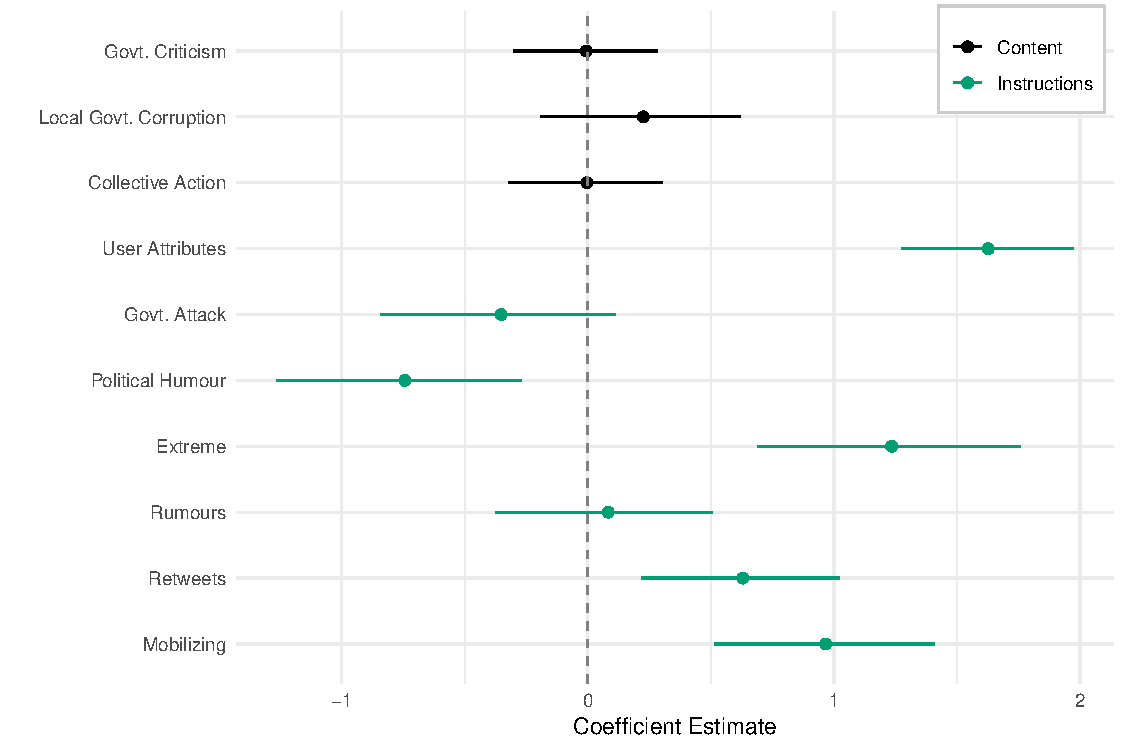
\includegraphics[width=\textwidth]{figures/coef_plot.pdf}\\
	\label{coef_plot}
\end{figure}
}

\paragraph{} The biggest predictors of whether or not content or users are ``reported up'' are the presence of words that describe the influence of the user mentioned in the log (User), and, to a lesser degree, how ``extreme'' the content is (Extreme). This would include content that is making exaggerated moral and emotional appeals or advocating extremist positions. Mentions of retweets and the degree to which a post ``incites'' (shandongxing, 煽动性) are also significantly and positively associated with whether a user is ``reported up.'' As we discuss in the cases below, this category would include posts that are inciting, even if only abstractly. It could include explicit exhortations for real-world social mobilization, but only if these exhortations incite or stir up strong emotions. By contrast, measured and journalistic statements of fact about collective action incidents would not fall into this category.

\paragraph{} No content-based independent variables were significant. The censors instead appear to focus on the framing of content, e.g., content that ``incites'' rather than  simply content about collective action events. For example, during an August 2012 taxi strike in the city of Hangzhou, the censors note, ``Hangzhou taxis are on a collective stoppage today, protesting the rise in gas prices and the state of the roads. This news can be circulated, but any posts that incite or appeal to other cities should be ``made secret.''\footnote{A type of ``shadow-banning,'' a censorship tactic where posts are hidden from a subset of users rather than deleted. When a post is ``made secret,'' the original poster can see it, but no one else can.} Report the original poster.'' Similarly, in logs about the 2013 arrest of Zhang Anni, the 12-year old daughter of a Tiananmen activist who wrote a letter to Barack Obama, the censors allow for discussion of the case, but not ``incitement'':

{\setstretch{1}
\epigraph{``Netizens expressing support for the Zhang Anni incident in Hebei, deal with any inciting content on Weibo, there is no need to delete general discussion at this point.''\footnotemark\newline}{--- Log entry from April 10, 2013}}
\footnotetext{Original Chinese: ``网友声援合肥张安妮事件,微博中处理煽动行动内容,一般讨论的暂时不必处理。''}

\paragraph{} The censors may realize that these are hot button topics, and deletion is not in their commercial interest. It is also possible the state itself is tolerant of more open discussion because while some will sympathize with the striking taxi drivers or young activists, others will criticize them for inconveniencing customers or being insufficiently patriotic. \cite{han2018contesting} argues that the state benefits from a more open online atmosphere because this allows ``discourse competition'' between supporters and opponents of the government. These posts reveal that thin line tread by the commercial censors. Sina tolerates discussion of collective action and political dissidents up to a point but reports it to the authorities if it ``incites.'' 
\paragraph{} The commercial censors report up information about influential ``big V'' users, and viral, inciting news. Online information control is deployed alongside real-world physical repression for the die-hard activists, as we see below in the case of Xu Zhiyong (许志永), the civil society activist.

\subsection{Selected Cases}

\paragraph{} In the section below, we discuss three emblematic cases of the phenomenon of ``reporting up.'' These cases are selected because they represent three areas of government concern: government legitimacy (Yang Lan's citizenship), political dissidence (Xu Zhiyong's arrest), and elite defection (Bo Xilai's trial). Only the second is a clear case of a call for collective mobilization against the state. As such, these cases demonstrate the significance of user characteristics across diverse areas of political sensitivity. 

\subsubsection{Yang Lan's Citizenship}

\paragraph{}On March 7, 2012, the censors at Weibo were getting off the night shift. As they wrote up guidance and instructions for the next shift, they wrote, ``Saying that Yang Lan is a US citizen has already been declared a rumor, directly delete posts of small users, report up big users.''\footnote{Original Chinese: 说杨澜是美国籍的已经辟谣了,小用户直接删除重要用户 报一下} A few days later, they repeated the command, ``[Suggesting that] ‘Yang Lan is a US citizen' should be considered fake news, if it is seen on Weibo, delete it, report big users.''\footnote{Original Chinese: 传杨澜为美国籍为虚假消息 微博见到删除 重点用户报一下.} 
\paragraph{} The censors were attempting to shut down a raging debate on Weibo, ``Is American citizenship still valuable?'' On March 6, there were more than 1.5 million posts on the topic. Some of the discussion focused on the post-Global Financial Crisis state of the US economy, but other Netizens took aim at their compatriots. ``If you say China isn't good, you are a Western slave. If you say America is good, you are an American bitch. If you say you don't want to be Chinese, you are a wretch and a traitor [...] If you get a green card and stand on the corner of American streets shouting, `I love you, China,' you are a `patriot.'\footnote{Archived Atlantic article available \href{https://web.archive.org/web/20170827203544/}{here}}
\paragraph{} Yang Lan (杨澜), a celebrity journalist and TV host, ``China's Oprah Winfrey,'' was alleged to be this kind of person. She appeared patriotic and had a strong political background (her father was a translator for Zhou Enlai), but after making a fortune in China's media market, she had taken citizenship elsewhere. Yang tried to rebut the accusations. Later, she and her wealthy husband, Bruno Wu, threatened to sue.
\paragraph{} In the Yang Lan case, the censors treated users differently based on how important and influential they are. Sina deleted normal users' posts when they gossiped about or criticized Yang Lan; they deleted the accounts and reported opinion leaders who did the same. While collective action may have been a concern in this case, it is more likely that the government was concerned about its legitimacy. If someone like Yang Lan, who is well-connected, wealthy, successful, and ``within-the-system'' is seeking foreign citizenship, it reflects poorly on the CCP. Are elites losing faith in the country's future? Do even the well-connected and wealthy have an exit option should the future take a turn for the worse? The crackdown on the Yang Lan case shuts down these questions.

\subsubsection{The Arrest and Trial of Xu Zhiyong}
\paragraph{} In cases involving well-known political activists, however, the concern with influence is more directly connected to social mobilization and collective action. For example, Xu Zhiyong, a well-known political activist and liberal reformer, first became famous in 2003 as part of a group of intellectuals who challenged the state's ``custody and repatriation system'' that detained rural migrants who did not have legal documentation to live in cities. He later opened an NGO, Open Constitution Initiative (Gongmeng, 公盟), which championed the rights of migrants to education in cities and investigated other scandals. He was detained in 2009 and Gongmeng was accused of tax evasion. At the time, Xu was working on the case of the tainted milk scandal in 2008, which had led to the deaths of several infants who consumed adulterated baby formula. In May and August of 2012, Xu Zhiyong used Weibo to ask for citizen support for Gongmeng, even soliciting donations online and calling for unity among Chinese citizens. Both of the posts below were instructed to be ``made secret,'' ``big V'' users who posted such material were reported up.

{\setstretch{1}
\epigraph{``On May 23rd, Xu Zhiyong used domestic sites (Sina Weibo and Tencent Weibo) and foreign sites (Twitter)  to incite Netizens to join {\it Gongmeng}, to purchase a ``citizen'' badge. Even calling for people to sign a ``citizen promise.'' [...] If this content is seen on Weibo, make it secret. Report big users to the authorities.''\footnotemark\newline}{--- Log entry from May 26, 2012}}
\footnotetext{Original Chinese: ``许志永''于5月23日在境内《新浪微博》、《腾讯微博》及境外《推特》发布 信息煽动网民加入``公盟''组织,购买``公民''徽章。并呼吁网民签署《公民承诺 》。原文称:``需要公民徽章的请给我发信 [EMAIL],我们需 要再订制。其实不需要传统意义上的所谓加入,公民(公盟)是自由公民的联 合,我们都是时代新公民,为公民社会共同努力!请发信至 [EMAIL],常联系。 这个内容微博中见到私密,重要用户发的上报负责人''}

{\setstretch{1}
\epigraph{``If 10,000 citizens each give {\it Gongmeng} 100 yuan, we could do so many things! We earnestly request support for {\it Gongmeng}; please believe we will use the money for the places that are most in need of justice. Legal aid assistance account: Xu Zhiyong, China Industrial Bank Beijing Branch, [BANK INFO] - Secret posts calling for donations to {\it Gongmeng}.''\footnotemark\newline}{--- Log entry from October 8, 2012}}
\footnotetext{Original Chinese: ``如果有一万个公民每年每人捐给公盟100元,我们能做多少事啊!恳请支持公盟,请相 信我们会把钱用到最渴求正义的地方。法律援助救助账号:许志永,中国工商银行北京 分行学院路支行,[BANK INFO],支付宝兼 恳请支持,望扩散 号召给公盟捐钱的私密''}
\paragraph{} In 2013, activists, including Xu Zhiyong, called for greater disclosure of government salaries and wealth. Xu Zhiyong championed this initiative as part of his new venture, The New Citizens Movement.\footnote{A more detailed analysis of this movement is in \cite{pils2014china}.} Demonstrations were held in several cities and led to the arrests of many people. After being under house arrest for three months, Xu Zhiyong was finally detained in July 2013, charged with ``attempting to disturb public order'' in August, and sentenced to four years in prison after a trial in January 2014. (He was released from prison in July 2017.)
\paragraph{} During this time of renewed activism around transparency issues, the commercial censors were given many orders to censor information about Xu Zhiyong and, importantly, to report up ``big users'' and ``special circumstances.'' Certain users were named in particular, including Xu's defense lawyer, Liu Weiguo, and other rights defense lawyers. On the same day of the post below, Liu was himself detained:

{\setstretch{1}
\epigraph{``Regarding the issue of several lawyers going to Beijing's Third Detention House to visit the detained Xu Zhiyong, when verifying, make [this information] secret. Increase the number of keywords that are automatically ``made secret.'' Immediately report up any special circumstances, including the lawyers, Chen Jiangang (陈建刚), and Liu Weiguo (刘卫国). These two say a lot. While verifying, pay careful attention; these words have already been verified.''\footnotemark\newline}{--- Log entry from July 18, 2013}}
\footnotetext{Original Chinese: ``关于有几位律师和网民去北京第三看守所看望被关押的许志永一事,审核中见到都私密处理,加了部分自动私密关键词,有特殊的情况及时上涉及的律师:陈建刚 刘卫国 这两个人说的比较多,审核的时候多注意,已经是审核词了''}
%\footnote{Read more about Chen Jiangang \href{https://web.archive.org/web/20170827210454/https://www.hongkongfp.com/2017/04/04/chinas-extraordinary-response-11-nation-letter-torture-human-rights-lawyers/}{here}}
%\footnote{Read more about Liu Weiguo \href{https://web.archive.org/web/20170827210526/http://www.scmp.com/news/china/policies-politics/article/1837022/about-50-human-rights-lawyers-and-law-firm-staff-held}{here}}

\paragraph{} With well-known political activists who openly challenge the government several fronts, the repressive apparatus of the state is not hidden or subtle. The commercial censors are told the issue is of great importance, and online discussion is used to monitor particular people, both virtually and eventually, through physical detention and criminal charges. Many of the lawyers mentioned in these posts were later detained in the July 2015 massive crackdown on human rights lawyers across China. Many other ``rights defense'' lawyers have gone underground since the arrests of 2014 and 2015 \citep{pils2014china}.

\paragraph{} The Xu Zhiyong incident reveals the government's desire to shape and guide public opinion, not just repress the actions of these few or stop collective action. During the January 2014 trial of Xu, for example, censors were instructed to calibrate censorship carefully:

{\setstretch{1}
\epigraph{``Tonight at the First Intermediate Court in Beijing, Wang Gongquan (王功权) admits guilt that he and Xu Zhiyong incited people to disturb public order, he has deeply reflected and awaits trial. Related content can be discussed as long as it reflects the media reports. Make secret anything that does not reflect the official line, stop small users and small media from discussing. Discussions in the big media should be verified first, posts with lots of retweets should be carefully reviewed.''\footnotemark\newline}{--- Log entry from January 22, 2014}}
\footnotetext{Original Chinese: ``王功权承认违法犯罪被取保候审 】北京市一中院今晚称,王功权承认与许志永策划煽动聚众扰乱公共场所秩序的违法犯罪活动,王功权表示深刻反省;对王功权予以取保候审。相关内容目前可以按照该新闻口径讨论,凡是与新闻不一致的私密处理,小用户小媒体禁止评论,大媒体评论先审转高审。''}

\paragraph{} Both the Yang Lan and Xu Zhiyong cases demonstrate the targeting of influential users as the regime seeks to control what is said and heard about China's elite. The cases are different in the sense that Yang Lan's citizenship is an abstract threat to the CCP's standing, while Xu Zhiyong's exhortation to fellow citizens is a concrete call for social mobilization. It is no coincidence that these cases involve a famous lawyer and even more famous journalist, part of China's new professionalized and cosmopolitan elite. It is critically important to the Party not only what they do or say online, but also what other people say about them. 

\subsubsection{Bo Xilai's Scandal}

\paragraph{} The importance of external elite voices was apparent during the 2012-2013 power struggle, and potential coup, which pitted Chongqing Party Secretary Bo Xilai and the incoming leader, Xi Jinping. As the scandal unfolded, influential users who expressed support for Bo were reported to the authorities. Additionally, the government demanded that Sina Weibo monitor and report public opinion data at fixed intervals. In the log below, we see Sina implementing requests to report data about public opinion related to Bo Xilai. This log serves both an informational role and a repressive role:

{\setstretch{1}
\epigraph{``Handling Bo Xilai-related posts: Total posts censored, among them, support for Bo (\#, \%), ridicule [of Bo] (\#, \%), reposting foreign media (\#, \%), other (\#, \%). [Also report] whether or not there are any influential users directly supporting Bo. Also, today's Bo Xilai reporting should be calculated according to the following intervals. The reporting up schedule has been revised to the following three time slots: 10:00, 18:00, and 23:00.''\footnotemark\newline}{--- Log entry from April 12, 2012}}
\footnotetext{Original Chinese: ``有关薄的处理数XX条,其中,支持薄XX条,占XX\%,调侃XX条,占XX\%,转发 外媒XX条,占XX\%,其他情况XX条,占XX\%。有无影响力大的用户明显直接挺薄内 容。 今天薄熙来的数同时按这个时段统计 这个报数时间段改为 10点、18点 、23点三时段''}

{\setstretch{1}
\epigraph{``[Keep track of the] number of deleted and filtered posts about Bo Xilai and Wang Lijun, the number of deleted and filtered comments, how many of these are articles oppose the way the central government has handled Bo Xilai, are unsatisfied with the results of the investigation of the case, how many are republished from foreign websites, and other related information. The reporting timeline has been changed as follows to these three times: 11:00, 16:00, and 23:00.''\footnotemark\newline}{--- Log entry from April 13, 2012}}
\footnotetext{Original Chinese: ``薄和王的删除、过滤数,共删除 条,过滤 条,其中反对中央对薄熙来处理决定的 篇;不满案件调查结果的 篇;转载境外网站的 篇;其他类信息 篇。11点、16点、23点三时段 以后时段更改如下。''}

\paragraph{} The Bo Xilai scandal was what the Party calls a ``sudden, unexpected emergency'' (tufa shijian, 突发事件). As such, immediate public opinion responses were followed with data collection and planning for more comprehensive public opinion interventions as the situation developed. More targeted interventions required information gathering, which is why Sina was asked to report data to the authorities. In later stages of the crisis, more specific topics of conversation became off-limits, not because there were pre-existing procedures to target specific categories of content, but because the goal of ``opinion guidance'' is to reduce the visibility and influence of content propagated by counter-hegemonic voices and increase the visibility of state narratives. An example is a more specific log from the Politburo Standing Committee's inspection tour of Chongqing following the incident:

{\setstretch{1}
\epigraph{``Today [MANAGER] published content moderation instructions for the inspection tour of Chongqing by the nine members of the Politburo Standing Committee (PSC):
\begin{enumerate}[noitemsep]
\item Manage all content (including news) related to the inspection tour of Chongqing by the nine members of the PSC.
\item Manage all rumors about government, the most important being: foreign reports and speculation, reports from foreign media where the size of discussion in the comment section is particularly large, content originating from sensitive individuals, commentary on Sina Online official accounts, and headline news.
\item For users who publish rumors, the Public Security Department will investigate and deal with the person at the time, and at the same time, investigate the criminal responsibility of the person in charge of the website.
\item In mid-May, government rumors were thoroughly cleaned up, and whenever one appeared, the owner of the website was required to go to a meeting at the city bureau and rectify their errors.''\footnotemark
\end{enumerate}
\strut
}{--- Log entry from April 27, 2012}}
\footnotetext{Original Chinese: ``今日[MANAGER]布置的九常委视察重庆的清理要求: 1:有关常委去重庆视察的内容(包括新闻,薄出事之前,所有微博账户)全部私密处理。薄被处理的新闻通稿不要动。 下周一前必须完成,做好分类的数据统计。常委名字+重庆、模式、唱红、打黑。 2:以后的时政谣言,从严处理,对用户必要时候上手段控制用户。 3:媒体评论,北京负责审核发现,及时报备,管理不住的常委新闻,就关闭评论,天津负责清理。 以上要求:监控所有人员务必执行。 通知原文: 
1:有关常委去重庆视察的内容(包括新闻)全部处理。 2:时政类谣言全部清理,主要类型为:外站报道及猜测、境内媒体的报道后面的评论及尺度比较大的一些新闻内容、敏感人士发布的内容、新浪网官方账户的评论,如头条新闻。 3:发布谣言的用户,公安部门将依法查处当时人,同时追究网站负责人的刑事责任。 4: 5月中旬彻底清理干净时政类谣言,凡出现一条,网站负责人必须去市局开会,进行整改。''}

\paragraph{} Later, as Bo Xilai was tried in the Jinan Intermediate People's Court, the logs portray a more planned and carefully executed opinion guidance strategy. Many China watchers expressed surprise when the Bo Xilai trial was covered live on Weibo, but this was done carefully and with Sina Weibo's cooperation.\footnote{See http://www.webcitation.org/74k5wmpno} On the opening day of the trial, Weibo was instructed to not only target categories of off-limits content but aid the Party in its efforts to set the agenda by heavily controlling counter-hegemonic discourse from ``Big V'' users and various non-official media accounts:

{\setstretch{1}
\epigraph{``... All comments discussing the matter from big media users and big V users are to be reviewed first before publication, one hour after the broadcast, lock comments. Directly prevent comments on small media accounts.''\footnotemark\newline}{--- Log entry from August 22, 2013}}
\footnotetext{Original Chinese: ``所有讨论此事的大媒体评论以及大V的评论均先审后上,一小时后锁定评论,小媒体发表此事直接关闭评论。''}

\paragraph{} In several related logs on the topic, content moderators were instructed to report up influential users and hide all content that was not exactly as reported by the Jinan Intermediate People's Court's Weibo account. By restricting discussion to official channels and focusing primarily on influential counter-hegemonic voices, the state was able to appear open, transparent, and legitimate in its trial of the fallen Party Secretary.

\paragraph{} In the handling of all three, Yang Lan's citizenship, Xu Zhiyong's trial, and the intrigue over the Bo Xilai affair, commercial censors delete or make secret information that mobilizes or incites public opinion, they report influential users to the authorities, and they also report up data on public opinion. Their tasks are multifaceted, and to focus only on the repressive activity misses the more sophisticated goals of guiding public opinion and delivering more accurate information to leaders about what opinion leaders and the masses are thinking regarding controversial topics. However, information about specific users can always be retained for future repressive activities. In an April 2011 log about a taxi and truck driver strike, the link between information and repression is apparent:

{\setstretch{1}
\epigraph{``Strengthen handling of inciting and harmful information about the taxi and truck drivers' strike against the rise in gas prices, especially information that mobilizes for the June 1 strike. Accumulate related news and retain the IP addresses (of users) with information that incites or mobilizes.''\footnotemark\newline}{--- Log entry from April 15, 2011}}
\footnotetext{Original Chinese: ``网监通知:进一步加强借``油价上涨''煽动出租车及货运司机罢运、罢工等的有害信息 的清理工作,特别是煽动6月1日罢工的信息。相关信息自行积累,行动性、煽动性信息查 IP留存。以便随时统计。昨日清理,目前未发现相关行动性信息。''}

\paragraph{} In an interview with the source of the leak, he recalls, ``when some political rumor was spread widely, or during the Tiananmen Square anniversaries, police harassed people based on the information we provided.'' The source recalls a manager once saying, ``hand in your big form. The police need it to arrest people'' when instructing employees at Sina Weibo's censorship office in Tianjin \citep{wang2016read,wang2016business}.

\section{Concluding Discussion}

\paragraph{} This paper contributes to our general understanding of the governance strategies of the Chinese Party-State in the virtual public sphere of social media. Building off earlier theories that emphasize the importance of limiting social elites external to the CCP, we find the government is concerned with the power of virality and influence on the Internet, a space that cannot be easily dominated simply via Communist Party organization. Attempts to mobilize citizens collectively via online discussions, such as in the Xu Zhiyong episode, are threats to the government's hold on power. However, the government attempts to limit ``counter-hegemonic discourse'' even when the threat of real-world collective action is not imminent. Work on social contention suggests that the Party may target influential thought leaders because they have large networks and can threaten information cascades that could undermine CCP legitimacy, encourage real-life collective action, or shift public opinion on important topics. Big-V users function as brokers by connecting social media users that previously may have had no connections. Large numbers of online followers create authority and discourse power that challenge CCP dominance.
\paragraph{} Maintaining responsiveness and more accurate monitoring of public opinion are essential facets of the government's strategy, however. In a sense, these findings underscore the information problems that confront dictators \citep{wintrobe2000political}. Social media discussion is desirable because it elucidates public opinion trends and social grievances. Nevertheless, it is also too much of a good thing.
\paragraph{} Going back to the exposition of the importance of Party leadership in \cite{schurmann1968ideology}, we confirm the CCP is most vociferously interested in constraining the rise of powerful alternative voices and influence. Schurmann's analysis is focused on the period when the old elite of the ancien regime is vanquished. Our focus is on a period when social media elevated new voices and allowed opinion leaders to re-emerge independent of the Party. Schurmann's perspective is still helpful, however, given its focus on the role of elites in leadership. The rise of the virtual public sphere created new challenges for the Party to maintain its discourse power and its organizational hegemony. As the newest battleground for the hearts and minds of citizens, social media platforms are critical spaces for the CCP to inhabit and dominate. New elite voices and opinion leaders must be co-opted or repressed.
\paragraph{} The government is intolerant of many topics once they become viral or are circulated by influential opinion leaders. The content of the post is less important than who is posting it and how many people are reposting it. The discussion over Yang Lan's citizenship, for example, seems to fall into this category. It does not immediately threaten any sort of collective action or revolt, but rather it is part of a gradual process in which the legitimacy of the Party is undermined and sabotaged by elites and influential thought leaders.
\paragraph{} Schurmann's work is instructive in part due to its focus on the 1950s, the period immediately after the Communist Revolution when the CCP was constructing the building blocks of its rule, and the 1960s, in the second edition, when social mobilization during the Cultural Revolution undermined the CCP's organizational dominance. In the realm of today's social media, the CCP is similarly limited in its capacity to take over all the space afforded by the Internet, nor does it wish to do so given the advantages of having more free discussion and better information about public opinion. Instead, the CCP focuses on repressing or co-opting voices that could threaten its position of leadership, to counter what \cite{lei2015contesting} call the ``counterhegemonic public sphere.'' This is an arena in which citizens are exposed to and generate discussion often beyond the confines of the official government position. The critical threat is not the degree to which public opinion is representative, but rather how influential one is. They write:

\begin{quote}
As the propaganda official put it, in the end, it is those who speak up instead of those who keep silent that influence other people and bring trouble for the Chinese government \cite[455]{lei2015contesting}.
\end{quote}

%\paragraph{} In a instructional guide written for government cadres called ``Governance Through Public Consultation on Weibo,'' online opinion leaders are listed as one of the main challenges to the regime \citep{zhang2014weibowenzheng}. Opinion leaders, according to the book, stand between the mass-media and the public. They have gained influence from the bottom-up and are less likely to be within the Party. In some cases, they are celebrities or self-made online forum stars. These opinion leaders can be harmful to regime interests because their response to an unforeseen event (a ``public opinion emergency'') can happen quickly with wide dissemination and influence.  Online influence can quickly turn into real-world significance, particularly if their voices are picked up by the traditional media. Rather than advocating for enhanced repression, the guide argues that the government should cultivate these leaders, reclaiming their influence through co-optation. If more opinion leaders identify with the Party, the Party can still set the agenda and play the lead role in any breaking story or crisis. 
\paragraph{} Despite the relevance of Schurmann's conceptualization of Party governance, it cannot fully capture the complex way in which the CCP manages virtual public spaces in a far more open, diverse, and vibrant context than experienced during the Maoist period. Moreover, more information and the ``appearance of freedom'' have real benefits to the government, both in terms of its legitimacy and its understanding of public opinion. \cite{repnikova2017media} finds the authorities shape media policy by carefully scouring social media. She finds, ``alongside control, Chinese authorities scrupulously listen to and study public opinion online, engage with and respond to public grievances, and creatively mobilize the public through interactive social media'' \citep{repnikova2018china}. \cite{stockmann2013media} shows that allowing for greater media liberalization with continued content control can bolster people's trust in the news. \cite{han2018contesting} argues, ``discourse competition'' between regime supporters and opponents benefits the state by revealing that Netizens are not all liberal CCP opponents. There are true believers, emboldened by the anonymity and the network-building available online. Finally, \cite{roberts2018censored} argues that censorship is more like a ``tax'' than a simple restriction on information. Most Netizens will never seek out sensitive political topics online or purchase a VPN to read foreign media. As these leaked blogs seem to indicate, the censors do indeed allow for a great deal of discussion online to happen while systematically targeting those few users who have the influence and the public following to cause real damage.
\newpage

\section*{Appendix}\label{appendix}

\subsection*{Logistic Regression Results}


\begin{table}[H] \centering 
  \caption{Logistic Regression Model for ``Reporting Up''} 
  \label{} 
\resizebox{!}{.35\paperheight}{\begin{tabular}{@{\extracolsep{5pt}}lc} 
\\[-1.8ex]\hline 
\hline \\[-1.8ex] 
 & \multicolumn{1}{c}{\textit{Dependent variable:}} \\ 
\cline{2-2} 
 & Report Up \\ 
\hline \\[-1.8ex] 
 Extreme & 1.234$^{***}$ \\ 
  & (0.272) \\ 
  Govt. Attack & $-$0.352 \\ 
  & (0.243) \\ 
  User Attributes & 1.627$^{***}$ \\ 
  & (0.178) \\ 
  Rumors & 0.083 \\ 
  & (0.224) \\ 
  Retweets & 0.630$^{***}$ \\ 
  & (0.206) \\ 
  Mobilizing & 0.967$^{***}$ \\ 
  & (0.228) \\ 
  Political Humor & $-$0.744$^{***}$ \\ 
  & (0.253) \\ 
  Govt. Criticism & $-$0.007 \\ 
  & (0.150) \\ 
  Local Govt. Corruption & 0.225 \\ 
  & (0.207) \\ 
  Collective Action & $-$0.004 \\ 
  & (0.160) \\ 
 \hline \\[-1.8ex] 
Observations & 2,212 \\ 
\hline 
\hline \\[-1.8ex] 
\textit{Note:}  & \multicolumn{1}{r}{$^{*}$p$<$0.1; $^{**}$p$<$0.05; $^{***}$p$<$0.01} \\ 
\end{tabular}} 
\end{table} 


\section*{Content Variables}


{\setstretch{1}
\begin{figure}[H]
	\centering
	\caption{Collective Action Coding Diagram}
	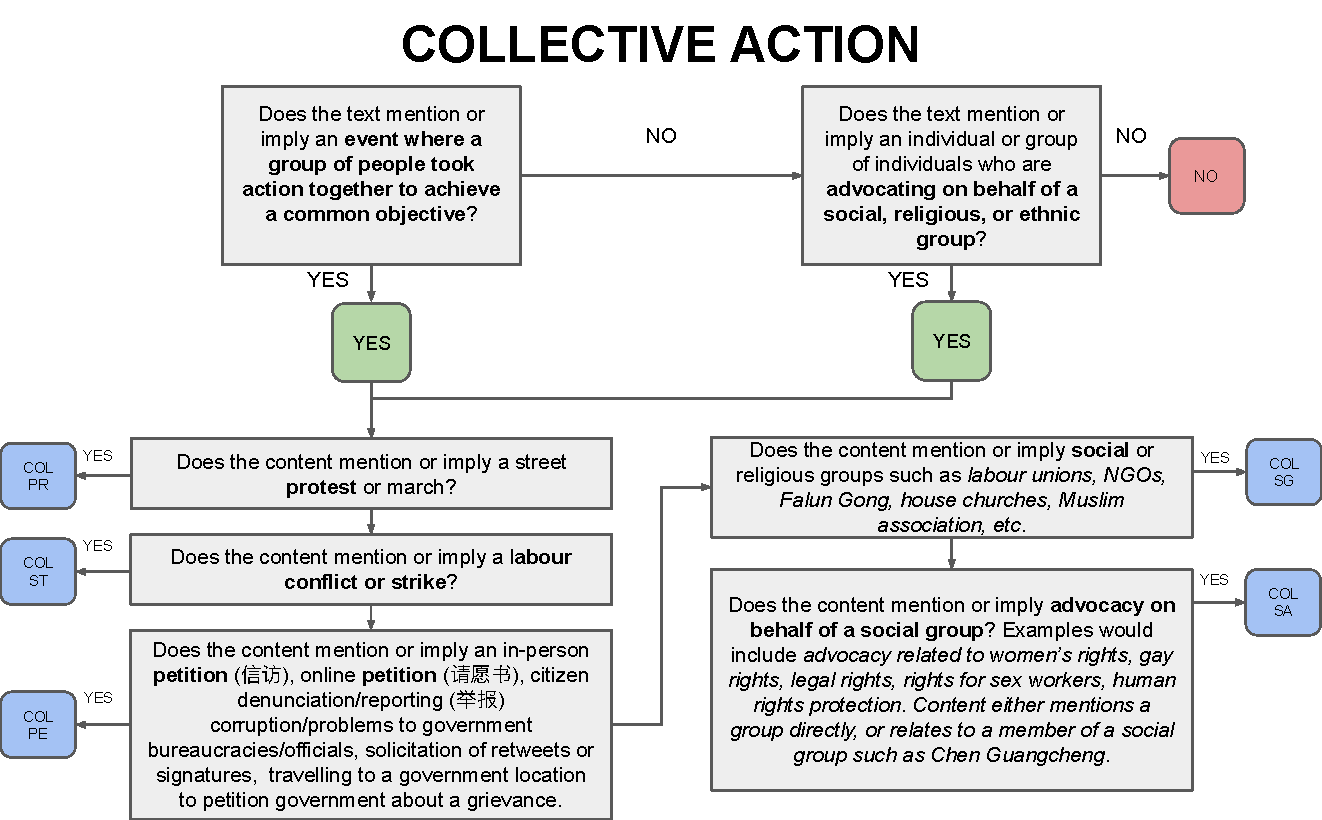
\includegraphics[width=\textwidth]{figures/coding_COL.pdf}\\
	\label{COL}
\end{figure}
}

{\setstretch{1}
\begin{figure}[H]
	\centering
	\caption{Corruption Coding Diagram}
	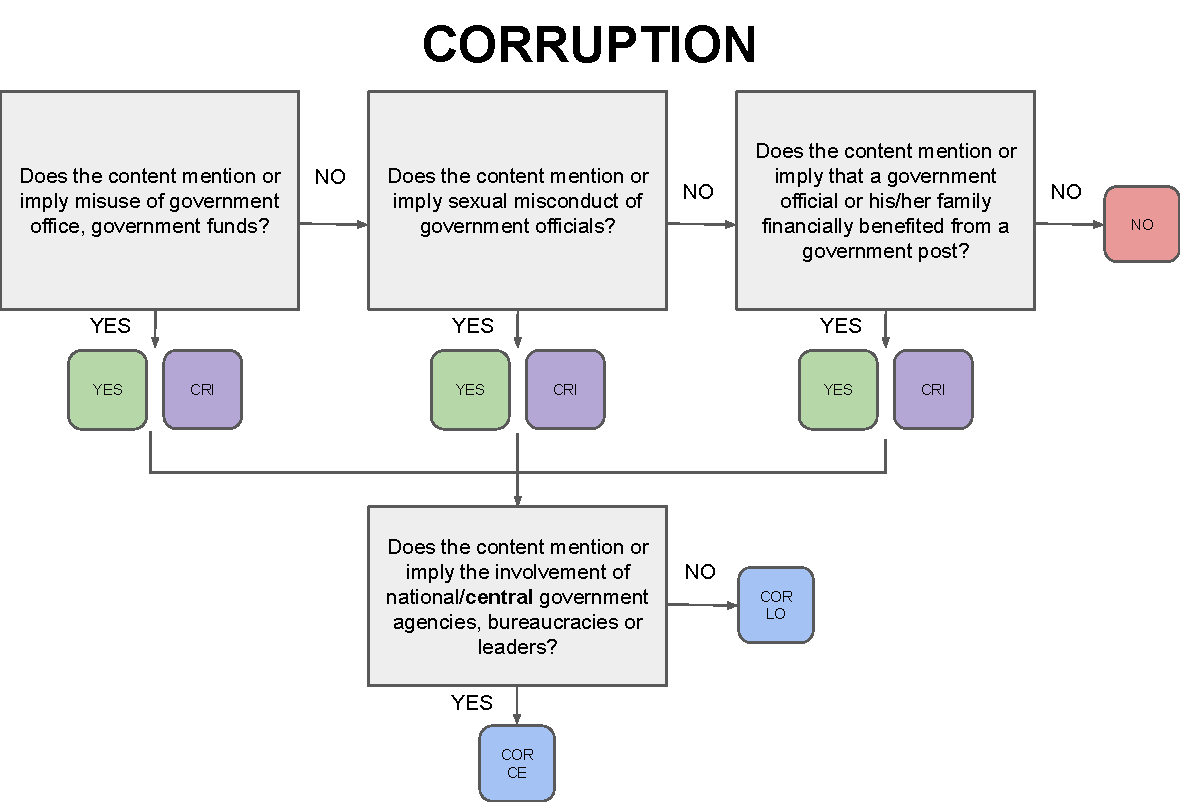
\includegraphics[width=\textwidth]{figures/coding_COR.pdf}\\
	\label{COR}
\end{figure}
}

{\setstretch{1}
\begin{figure}[H]
	\centering
	\caption{Government Coding Diagram}
	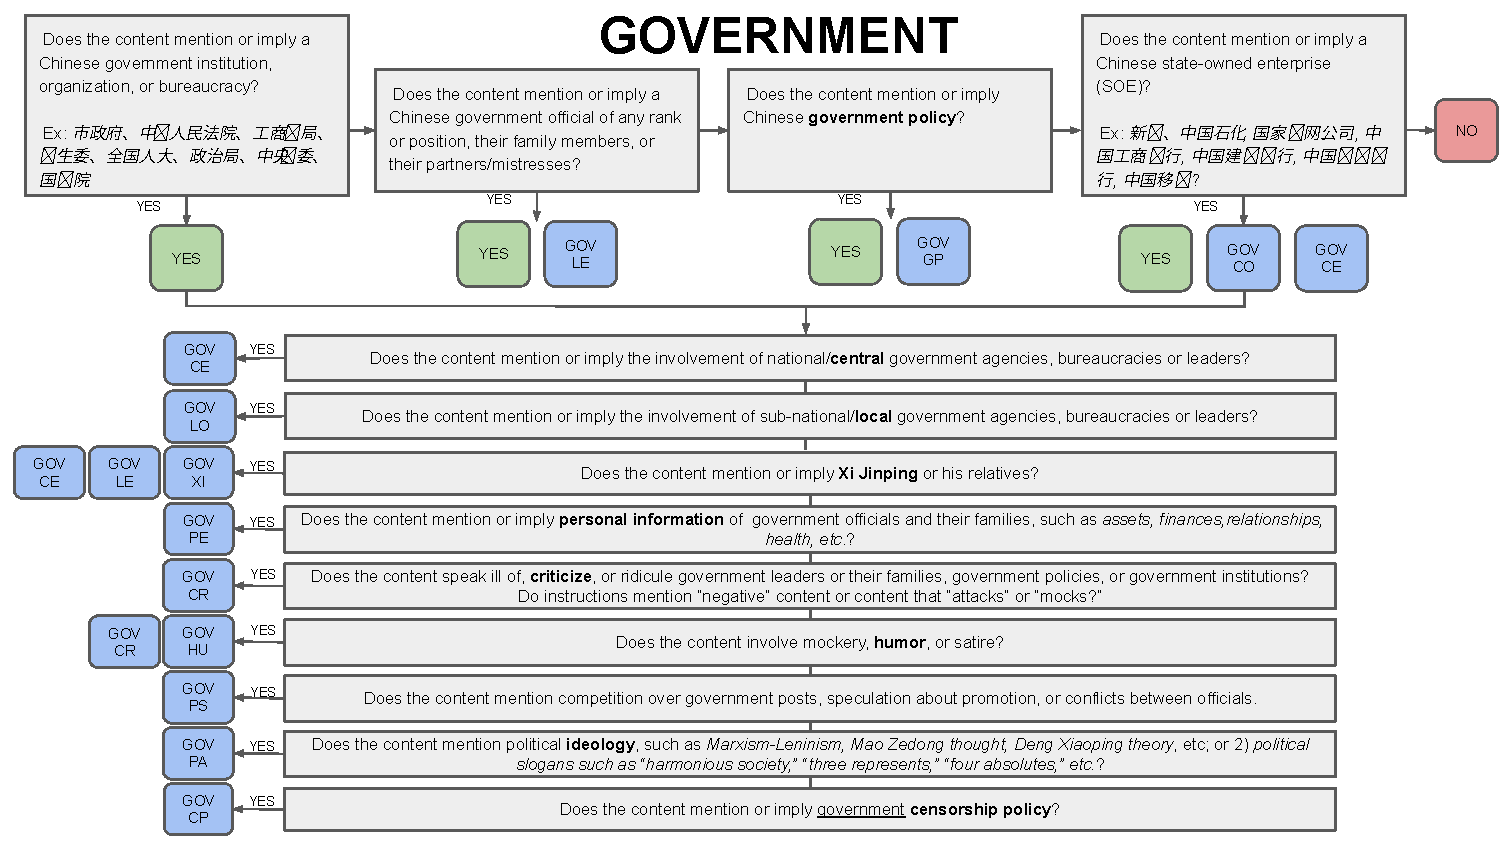
\includegraphics[width=\textwidth]{figures/coding_GOV.pdf}\\
	\label{GOV}
\end{figure}
}

\section*{Instruction Variables}

\subsection{Report Users}

The instruction text contains a (near) match of the following phrases used about a user (用户, UID):
\begin{itemize}[noitemsep]
	\item Report (报备, 报一下)
	\item Report up (上报)
	\item Send to Beijing (发给北京)
	\item Send it to the authorities (发给负责人, 提供给负责人)
\end{itemize}

\subsection{Report Data}

The instruction text contains a (near) match of the following phrases used about content (信息, 内容, 文章号, 言论, 评论):

\begin{itemize}[noitemsep]
	\item Report (报备, 报一下)
	\item Report data (报数)
	\item Report up (上报)
	\item Send to Beijing (发给北京)
	\item Send it to the authorities (发给负责人, 提供给负责人)
\end{itemize}

\subsection{User Attributes}

The instruction text contains a (near) match of the following attributes of users (用户, 账号, 号):

\begin{itemize}[noitemsep]
	\item Small [user] (小[用户,号])
	\item Big [user] (大[用户,号])
	\item Big V user---verified user with many fans, V---verified user, VIP (大V, V, VIP)
	\item Opinion leaders (意见领袖)
	\item Famous people (名人)
	\item \text{Media [users] (媒体)}
	\item Grassroots (草根)
	\item Important [users] (重要)
	\item Ordinary [users] (普通)
	\item Delete for ordinary users and make secret for verified users (普删V私)
	\item \text{[Users] with many fans (粉丝较多的)}
	\item \text{[Users] with around [\#] fans (粉丝数[\#]左右的)}
	\item \text{Newly-registered [accounts/users] (新注册)}
	\item Old accounts (老账户)
	\item Leftist [users] (左派)
	\item Rightist [users] (右派)
	\item \text{[Users] who post memes (段子类)}
	\item ``Reincarnated'' [users]---users who continually create new accounts after deletion (转世)
	\item \text{[Users] who continue to post (连续发布的用户)}
\end{itemize}

\subsection{Extreme}

The instruction text contains a (near) match of the following phrases used about content (信息, 内容, 文章号, 言论, 评论):

\begin{itemize}[noitemsep]
	\item Extreme (过激的)
	\item Excessive/overboard (过分的)
	\item Vicious/malicious (恶毒的)
	\item Malicious (恶意的)
	\item Disgusting/gross (恶性的)
	\item Disgusting/abominable (恶劣的)
	\item Inappropriate (不行的)
	\item Attacking (攻击的)
	\item Hurling invective (谩骂的)
\end{itemize}

\subsection{Attacking the Government}

The instruction text contains a (near) match of the following phrases used about content the country, the party, the internet management system, the party, party-state, country, government, system, social system, leadership, the Central Propaganda Department, Xi Jinping (我国, 我党, 我互联网管理制度, 党, 党政, 国家, 政府, 体制, 社会制度, 领导人, 中宣部, 习近平)

\begin{itemize}[noitemsep]
	\item Attack $\rule{1cm}{0.15mm}$ (攻击$\rule{1cm}{0.15mm}$)
	\item Make a negative connection with $\rule{1cm}{0.15mm}$ (负面联系$\rule{1cm}{0.15mm}$)
	\item Concerning something negative about $\rule{1cm}{0.15mm}$ (涉及$\rule{1cm}{0.15mm}$负面的)
\end{itemize}


\subsection{Rumors/Fake news}

The instruction text contains a (near) match of the following phrases used about content (信息, 内容, 文章号, 言论, 评论):

\begin{itemize}[noitemsep]
	\item Fake (虚假)
	\item Untrue information (内容不实)
	\item Spreading fake news (传播虚假消息)
	\item Spreading rumors (造谣)
	\item Unconfirmed true or false (不确定真假)
	\item According [to rumors] (传)
	\item Refuting rumors (辟谣的)
\end{itemize}

\subsection{Retweets}

The instruction text contains a (near) match of the following phrases used about content (信息, 内容, 文章号, 言论, 评论):

\begin{itemize}[noitemsep]
	\item Retweets cannot surpass [\#] (转发不能过[\#])
	\item Retweets surpass [\#] (转发超过[\#]的)
	\item Lots of retweets (转发多的, 转发高的, 转发较高的)
	\item Every hour surpassing [\#] retweets (每小时总量超过[\#])
	\item Pay attention to retweets (注意转发)
	\item Severely restrict retweets (严禁转载)
	\item Negative retweets (负面转发)
\end{itemize}

\subsection{Inciting}

The instruction text contains a (near) match of the following phrases used about content (信息, 内容, 文章号, 言论, 评论):

\begin{itemize}[noitemsep]
	\item Inciting (煽动性)
	\item Mobilizing (行动性)
	\item Collective (群体性)
	\item Call on/appealing to (号召的)
	\item Cause a fuss, make a scene (闹事)
	\item Causing a panic (造成恐慌的)
\end{itemize}

\subsection{Political Humor}

The instruction text contains a (near) match of the following phrases used about the country, the party, the internet management system, the party, party-state, country, government, system, social system, leadership, the Central Propaganda Department, Xi Jinping (我国, 我党, 我互联网管理制度, 党, 党政, 国家, 政府, 体制, 社会制度, 领导人, 中宣部, 习近平):

\begin{itemize}[noitemsep]
	\item Make fun of $\rule{1cm}{0.15mm}$ (拿$\rule{1cm}{0.15mm}$开玩笑)
	\item Ridicule (调侃)
	\item Satirize (讽刺的)
	\item Meme/joke (段子)
	\item Satirical humor(恶搞)
\end{itemize}


\subsection*{Intercoder Reliability}

\paragraph{} These are the results comparing the predictive power of coder 1 to coder 2's decisions using the area under the receiver operator curve (ROC AUC). All categories are above the acceptable measure of .7 and many are above .85, which is highly reliable. We also prevent another similar measure, Krippendorf's Alpha, which also shows reliability of the relevant categories. 

\begin{table}[hbt!]
	\caption{Intercoder Reliability Measures}
	\label{icr}
	\centering
	\begin{tabular}{|l|c|c|c|}
		\hline
		\textbf{Category} & \textbf{\% Agreement} & \textbf{AUC} & \textbf{Krip. Alpha} \\ \hline
		Col. Action & 0.90 & 0.88 & 0.76 \\ \hline
		%Petition & 0.95 & 0.78 & 0.64 \\ \hline
		%Protest & 0.89 & 0.84 & 0.68 \\ \hline
		%Social Activism & 0.93 & 0.82 & 0.67 \\ \hline
		%Social Groups & 0.97 & 0.86 & 0.59 \\ \hline
		%Strike/Labor Disputes & 1.00 & 1.00 & 1.00 \\ \hline
		Corruption & 0.95 & 0.93 & 0.86 \\ \hline
		%Central Corr. & 0.95 & 0.91 & 0.85 \\ \hline
		Local Corr. & 0.95 & 0.88 & 0.79 \\ \hline
		%Crime & 0.83 & 0.82 & 0.65 \\ \hline
		%Financial Crime & 0.95 & 0.92 & 0.86 \\ \hline
		%Illicit Goods and Services & 0.97 & 0.88 & 0.76 \\ \hline
		%Police & 0.93 & 0.85 & 0.58 \\ \hline
		%Violent Crime & 0.92 & 0.84 & 0.60 \\ \hline
		%Disaster & 0.91 & 0.90 & 0.65 \\ \hline
		%Man-made Disaster & 0.92 & 0.90 & 0.64 \\ \hline
		%Natural Disaster & 0.99 & 0.83 & 0.66 \\ \hline
		%Ethnic Groups & 0.97 & 0.98 & 0.85 \\ \hline
		%Foreign Media & 0.91 & 0.85 & 0.73 \\ \hline
		Govt. & 0.90 & 0.84 & 0.69 \\ \hline
		%Central Govt. & 0.83 & 0.83 & 0.65 \\ \hline
		%SOEs & 0.96 & 0.80 & 0.61 \\ \hline
		%Censorship Policy & 0.91 & 0.63 & 0.34 \\ \hline
		Govt. Criticism & 0.83 & 0.82 & 0.65 \\ \hline
		%Govt. Policy & 0.78 & 0.72 & 0.44 \\ \hline
		%Humor, Satire & 0.98 & 0.95 & 0.87 \\ \hline
		%Govt. Leadership & 0.93 & 0.93 & 0.85 \\ \hline
		%Local Govt. & 0.77 & 0.75 & 0.50 \\ \hline
		%Party Ideology & 0.95 & 0.81 & 0.31 \\ \hline
		%Personal Life of Leaders & 0.92 & 0.77 & 0.64 \\ \hline
		%Power Struggle & 0.89 & 0.63 & 0.35 \\ \hline
		%Xi Jinping & 0.96 & 0.98 & 0.75 \\ \hline
		%Hong Kong, Macau, and Taiwan & 0.95 & 0.97 & 0.73 \\ \hline
		%Nationalism & 0.89 & 0.78 & 0.64 \\ \hline
		%Rumor/Fake News & 0.93 & 0.91 & 0.69 \\ \hline
		%Sensitive Anniversary & 0.95 & 0.89 & 0.69 \\ \hline
		%Reoccurring Pol. Event & 0.95 & 0.66 & 0.34 \\ \hline
	\end{tabular}
\end{table}
\newpage

\newpage
\bibliographystyle{apacite}
\bibliography{repression}

\end{CJK*}
\end{document}
